\documentclass[a4paper,12pt]{report}
\usepackage{graphicx}
\usepackage{amsmath}
\usepackage{amsfonts}
\usepackage{amssymb} 
\usepackage{hyperref}
\usepackage{geometry}
\usepackage{multirow}
\usepackage{float}

\geometry{top=2cm,bottom=2cm,left=2cm,right=2cm}

\title{Merge Sort in OpenMP}
\author{
    % name and ID using tabular
    \begin{tabular}{ll}
        JIALI CLAUDIO, HUANG & Personal code: \underline{11032111} \\
        Peng, Rao & Personal code: \underline{11022931} \\
    \end{tabular}
}
\date{}

\begin{document}
\maketitle
\section*{Experimental setup}
We have implemented the merge sort algorithm in C++ using OpenMP. The code is compiled using the GCC compiler. The code is run on a machine with the following specifications:
\begin{table}[H]
    \caption{Experimental setup}
    \centering
    \begin{tabular}{c c}
        \hline
        Machine           & MacOS with Apple M1 pro chip(8 cores) \\
        Compiler Option   & g++14 -fopenmp -O3                    \\
        OMP\_NUM\_THREADS & 10                                    \\
        OMP\_SCHEDULE     & static                                \\
        \hline
    \end{tabular}
\end{table}

\section*{Performance measurements}
We have measured the performance of the merge sort algorithm by varying the size of the input array and the deep of the Parallelism. The performance is measured in terms of the execution time of the algorithm. The results are shown in the following tables and figures.
\begin{table}[H]
    \caption{Execution time of merge sort algorithm with different input sizes and depth}
    \centering
    \begin{tabular}{c c c}
        \hline
        Input size & Depth & Execution time (s) \\
        \hline
        $10^3$     & 5     & 0.000833           \\
        $10^3$     & 8     & 0.0001             \\
        $10^3$     & 10    & 0.0001             \\
        $10^4$     & 5     & 0.0001             \\
        $10^4$     & 8     & 0.0001             \\
        $10^4$     & 10    & 0.0001             \\
        $10^5$     & 5     & 0.0001             \\
        $10^5$     & 8     & 0.0001             \\
        $10^5$     & 10    & 0.0001             \\
        $10^6$     & 5     & 0.0001             \\
        \hline
    \end{tabular}
    \hfil
    \begin{tabular}{c c c}
        \hline
        Input size & Depth & Execution time (s) \\
        \hline
        $10^6$     & 8     & 0.0001             \\
        $10^6$     & 10    & 0.0001             \\
        $10^7$     & 5     & 0.0001             \\
        $10^7$     & 8     & 0.0001             \\
        $10^7$     & 10    & 0.0001             \\
        $10^8$     & 5     & 0.0001             \\
        $10^8$     & 8     & 0.0001             \\
        $10^8$     & 10    & 0.0001             \\
        $10^9$     & 5     & 0.0001             \\
        $10^9$     & 8     & 0.0001             \\
        \hline
    \end{tabular}
\end{table}
\begin{figure}[H]
    \centering
    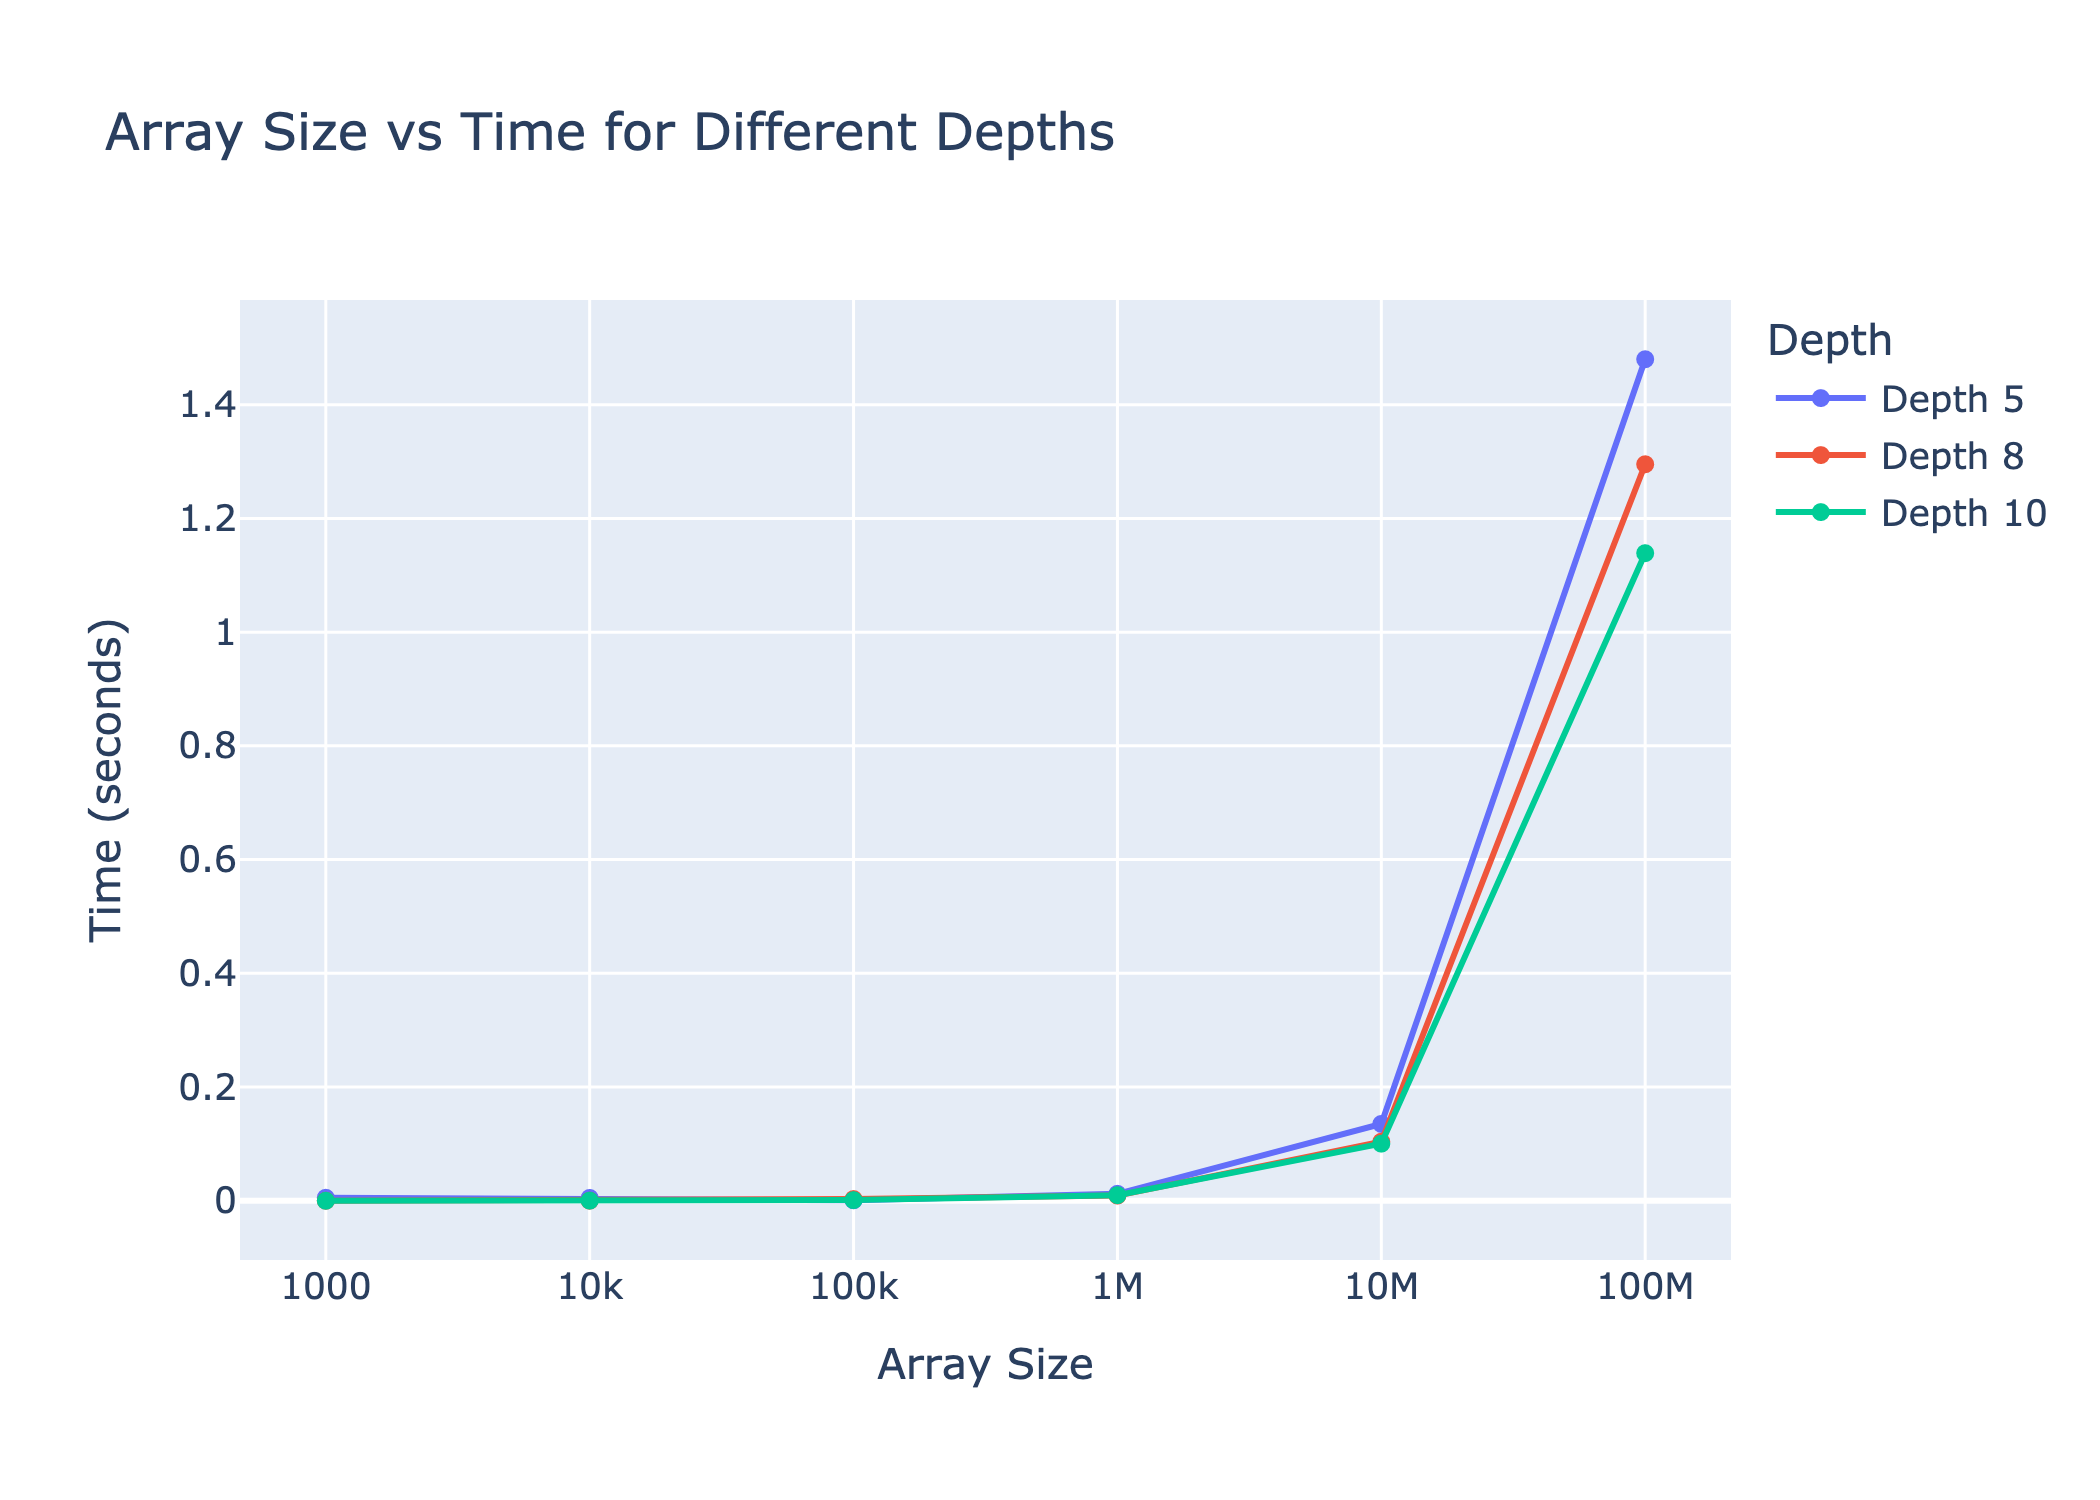
\includegraphics[height=0.32\textheight]{/Users/raopend/Workspace/PC_challenge/high_res_plot.png}
    \caption{Execution time of merge sort algorithm with different input5sizes and depth}
\end{figure}
\section*{Explanation of design choices}
The merge sort algorithm is a divide-and-conquer algorithm that including two main steps: divide and merge. So we can parallelize the divide step and merge step separately. This is the method of \textit{Introduce to Algorithm}\cite{cormen2001introduction}

\noindent\textbf{Design of OpenMP parallelization:}
\begin{itemize}
    \item We used the omp task method for parallelization. Because of the iteration of recursion is unknown, so we used the omp task method for parallelization.
    \item Use depth limited mechanism to prevent too much task generated to block threads.
    \item When the array size <= 800, it is more efficient sort by serial, so we used the cutoff mechanism to get better performance.
    \item Use omp\_get\_max\_threads() function to get threads dynamically so that it can perform well in different computer.
    \item In the merge sort algorithm, the scale of each recursion is similar, so we set schedule to static to avoid unnecessary operate.
\end{itemize}

\noindent\textbf{Design of the division:}
\begin{itemize}
    \item We divided the array into two parts and then recursively divided the two parts into two parts until the size of the array is less than or equal to 800.
    \item We used the omp task method to parallelize the division step.
    \item We used the depth limited mechanism to prevent too much task generated to block threads.
\end{itemize}

\noindent\textbf{Design of the merge:}
\begin{itemize}
    \item We used the omp task method to parallelize the merge step.
    \item We used the depth limited mechanism to prevent too much task generated to block threads.
    \item We used binary search to find the position of the element in the right part of the array.
\end{itemize}
\bibliographystyle{plain}
\bibliography{references}
\end{document}